%\section{Scénario d'utilisation}
\chapter{Scénario d'utilisation}
\markboth{\MakeUppercase{Scénario d'utilisation}}{}     

	\section{Aspect général}

		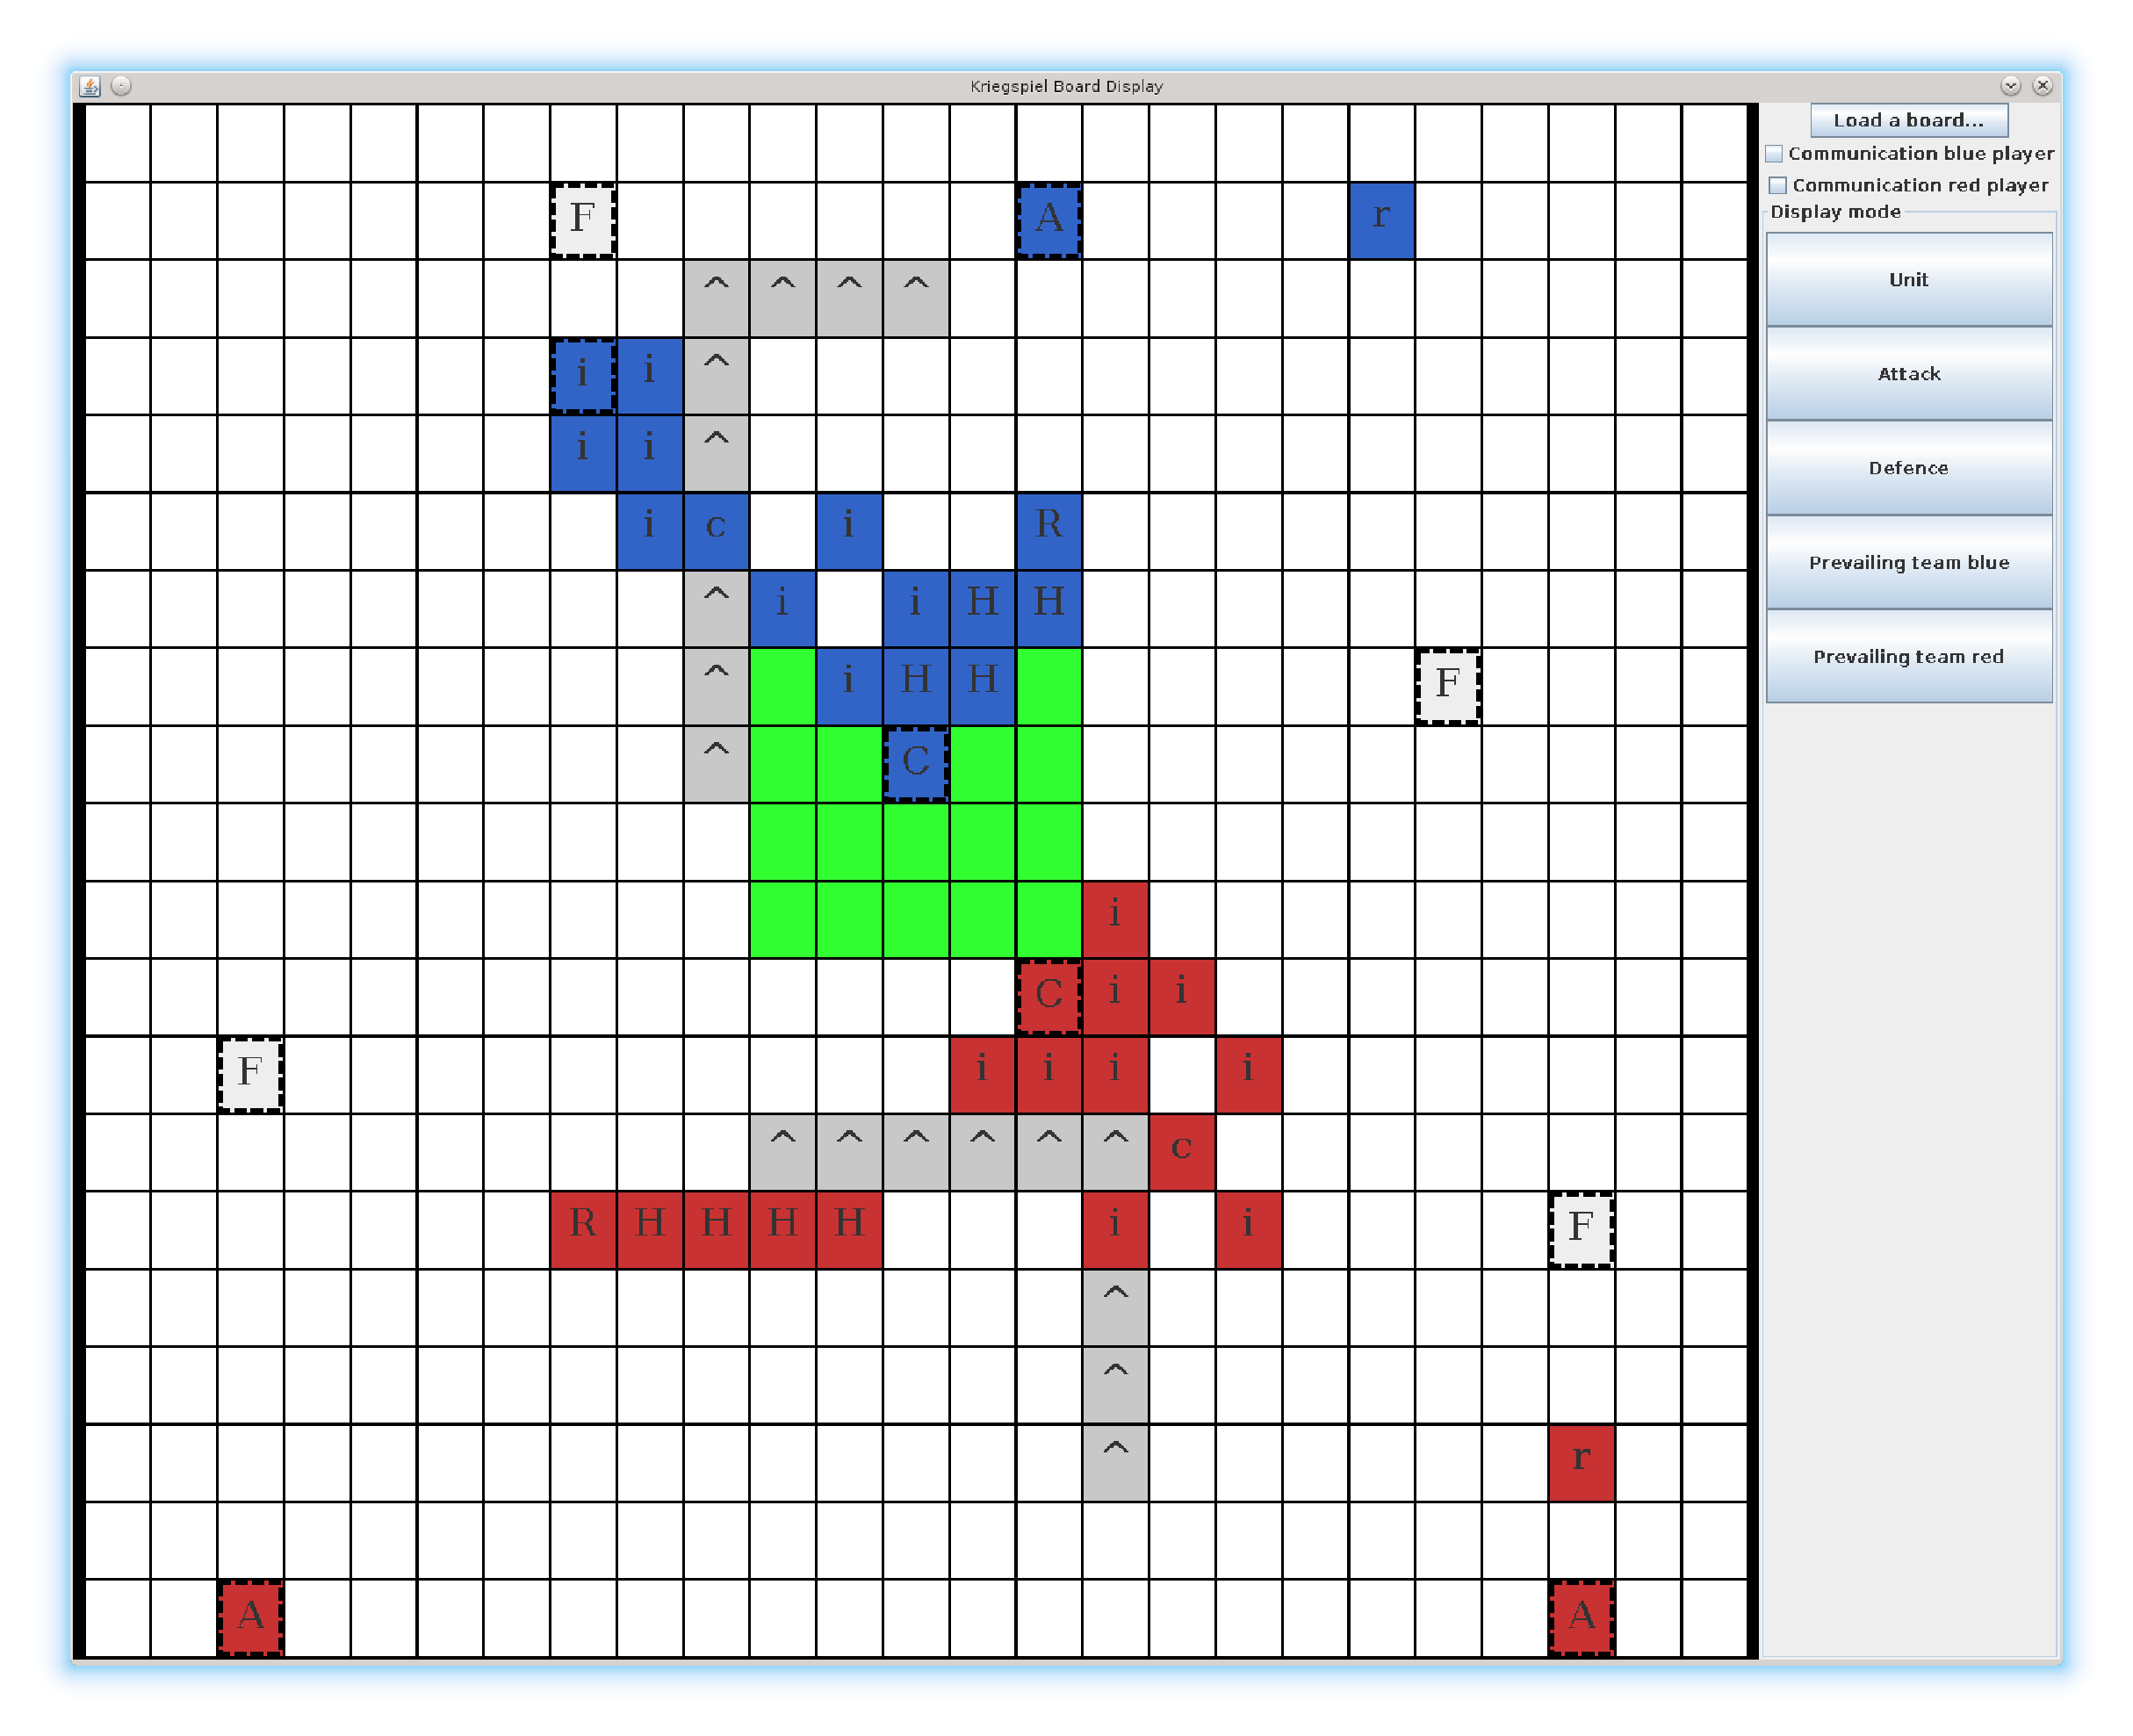
\includegraphics[scale=0.4]{images/screen1.eps}
		
		\paragraph{Le plateau :}
			L'affichage du plateau prend la majorité de la fenêtre.
			Les entités sont représentées par des lettres dans des cases de la couleur de leur équipe.
			Les \^{} sur fond gris sont les montagnes.
			Les cases possédant une bordure pointillée noire sont les entités qui peuvent contenir une autre entité	(les arsenaux et les forts).
			Les cases vertes représentent les possibilités de mouvement	de l'entité sélectionnée (ici le SwiftCanon bleu). 
			Notons que l'unité ne peut pas se déplacer sur une case déja occupée.
			Lorsqu'une entité risque d'être détruite au prochain tour, son symbole est entouré de ( ).
			Lorsqu'elle est forcée de se retirer au prochain tour, son symbole est entouré de [ ].
	
		\paragraph{Le menu :}
	
			Le menu contient différents éléments :
			- Le bouton de chargement en haut permet de charger une situation depuis un fichier?
			- Les checkboxes permettent d'activer ou de désactiver les communications
			- Les grands boutons permettent de changer le mode d'affichage

	\section{Les modes d'affichage}

		\subsection{Mode unités}
			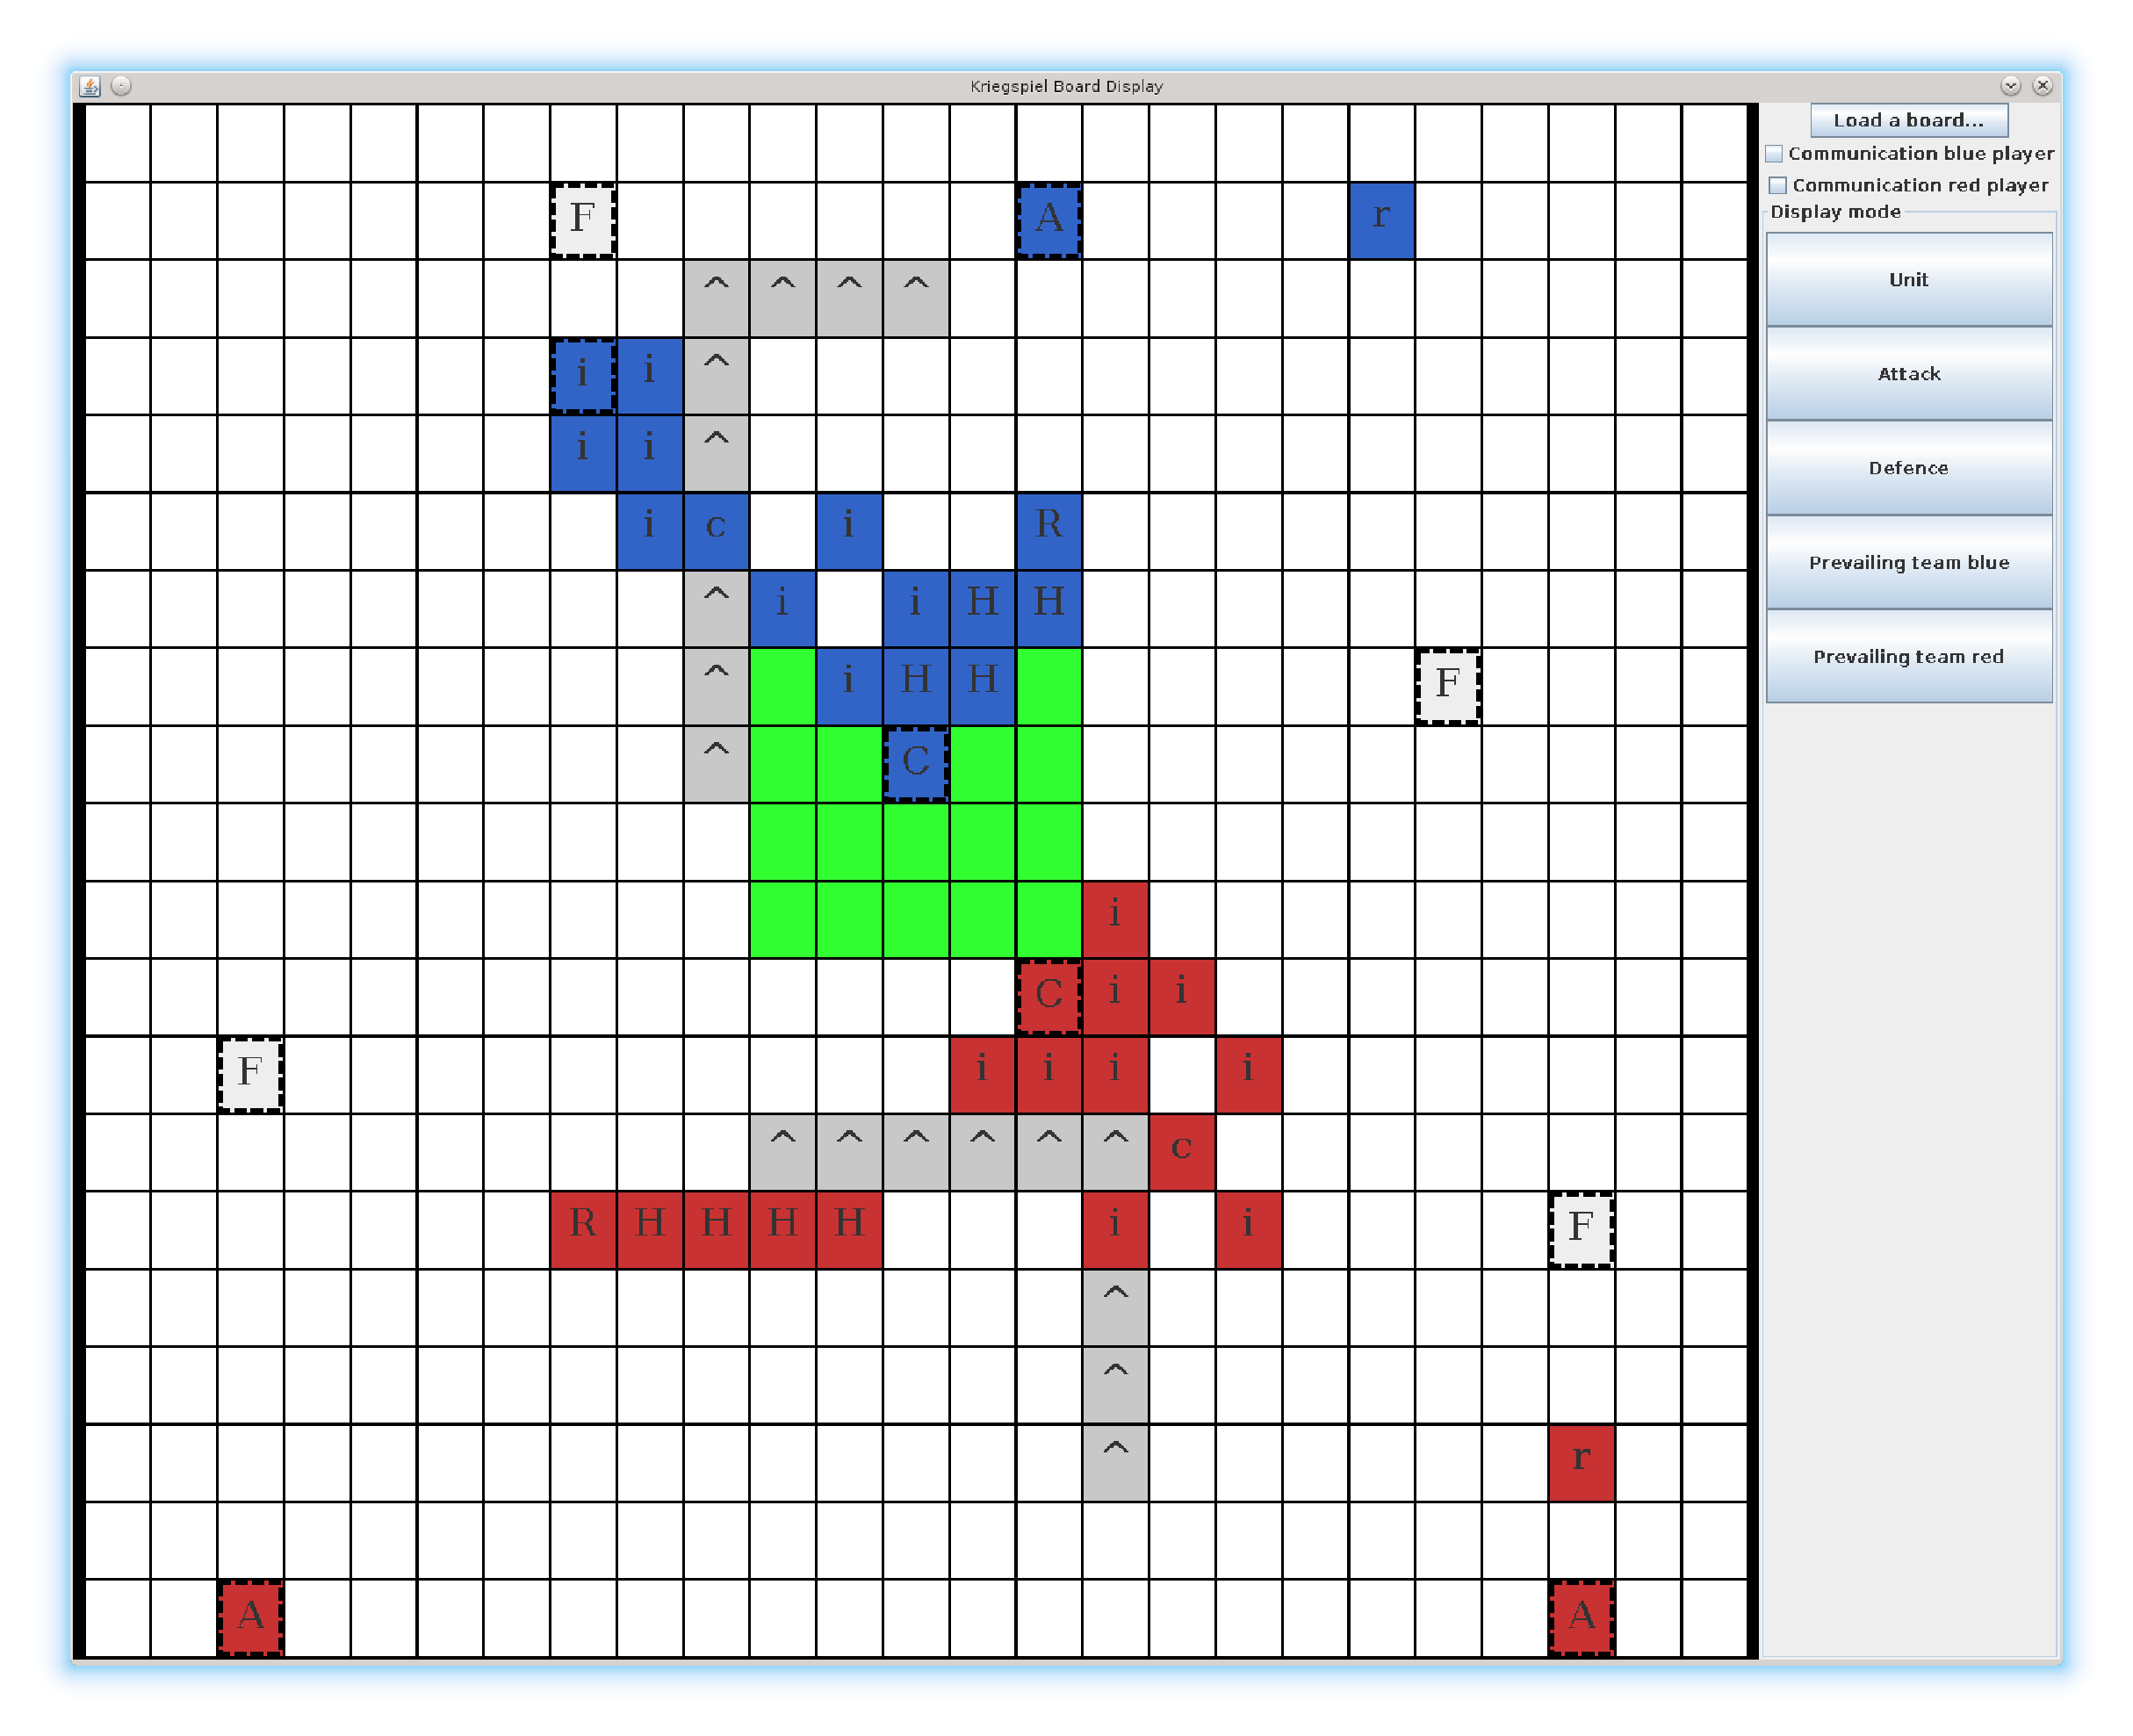
\includegraphics[scale=0.4]{images/screen1.eps}
			C'est le mode d'affichage principal, les symboles des unités sont affichés.

			\clearpage

		\subsection{Modes attaque/défense}
			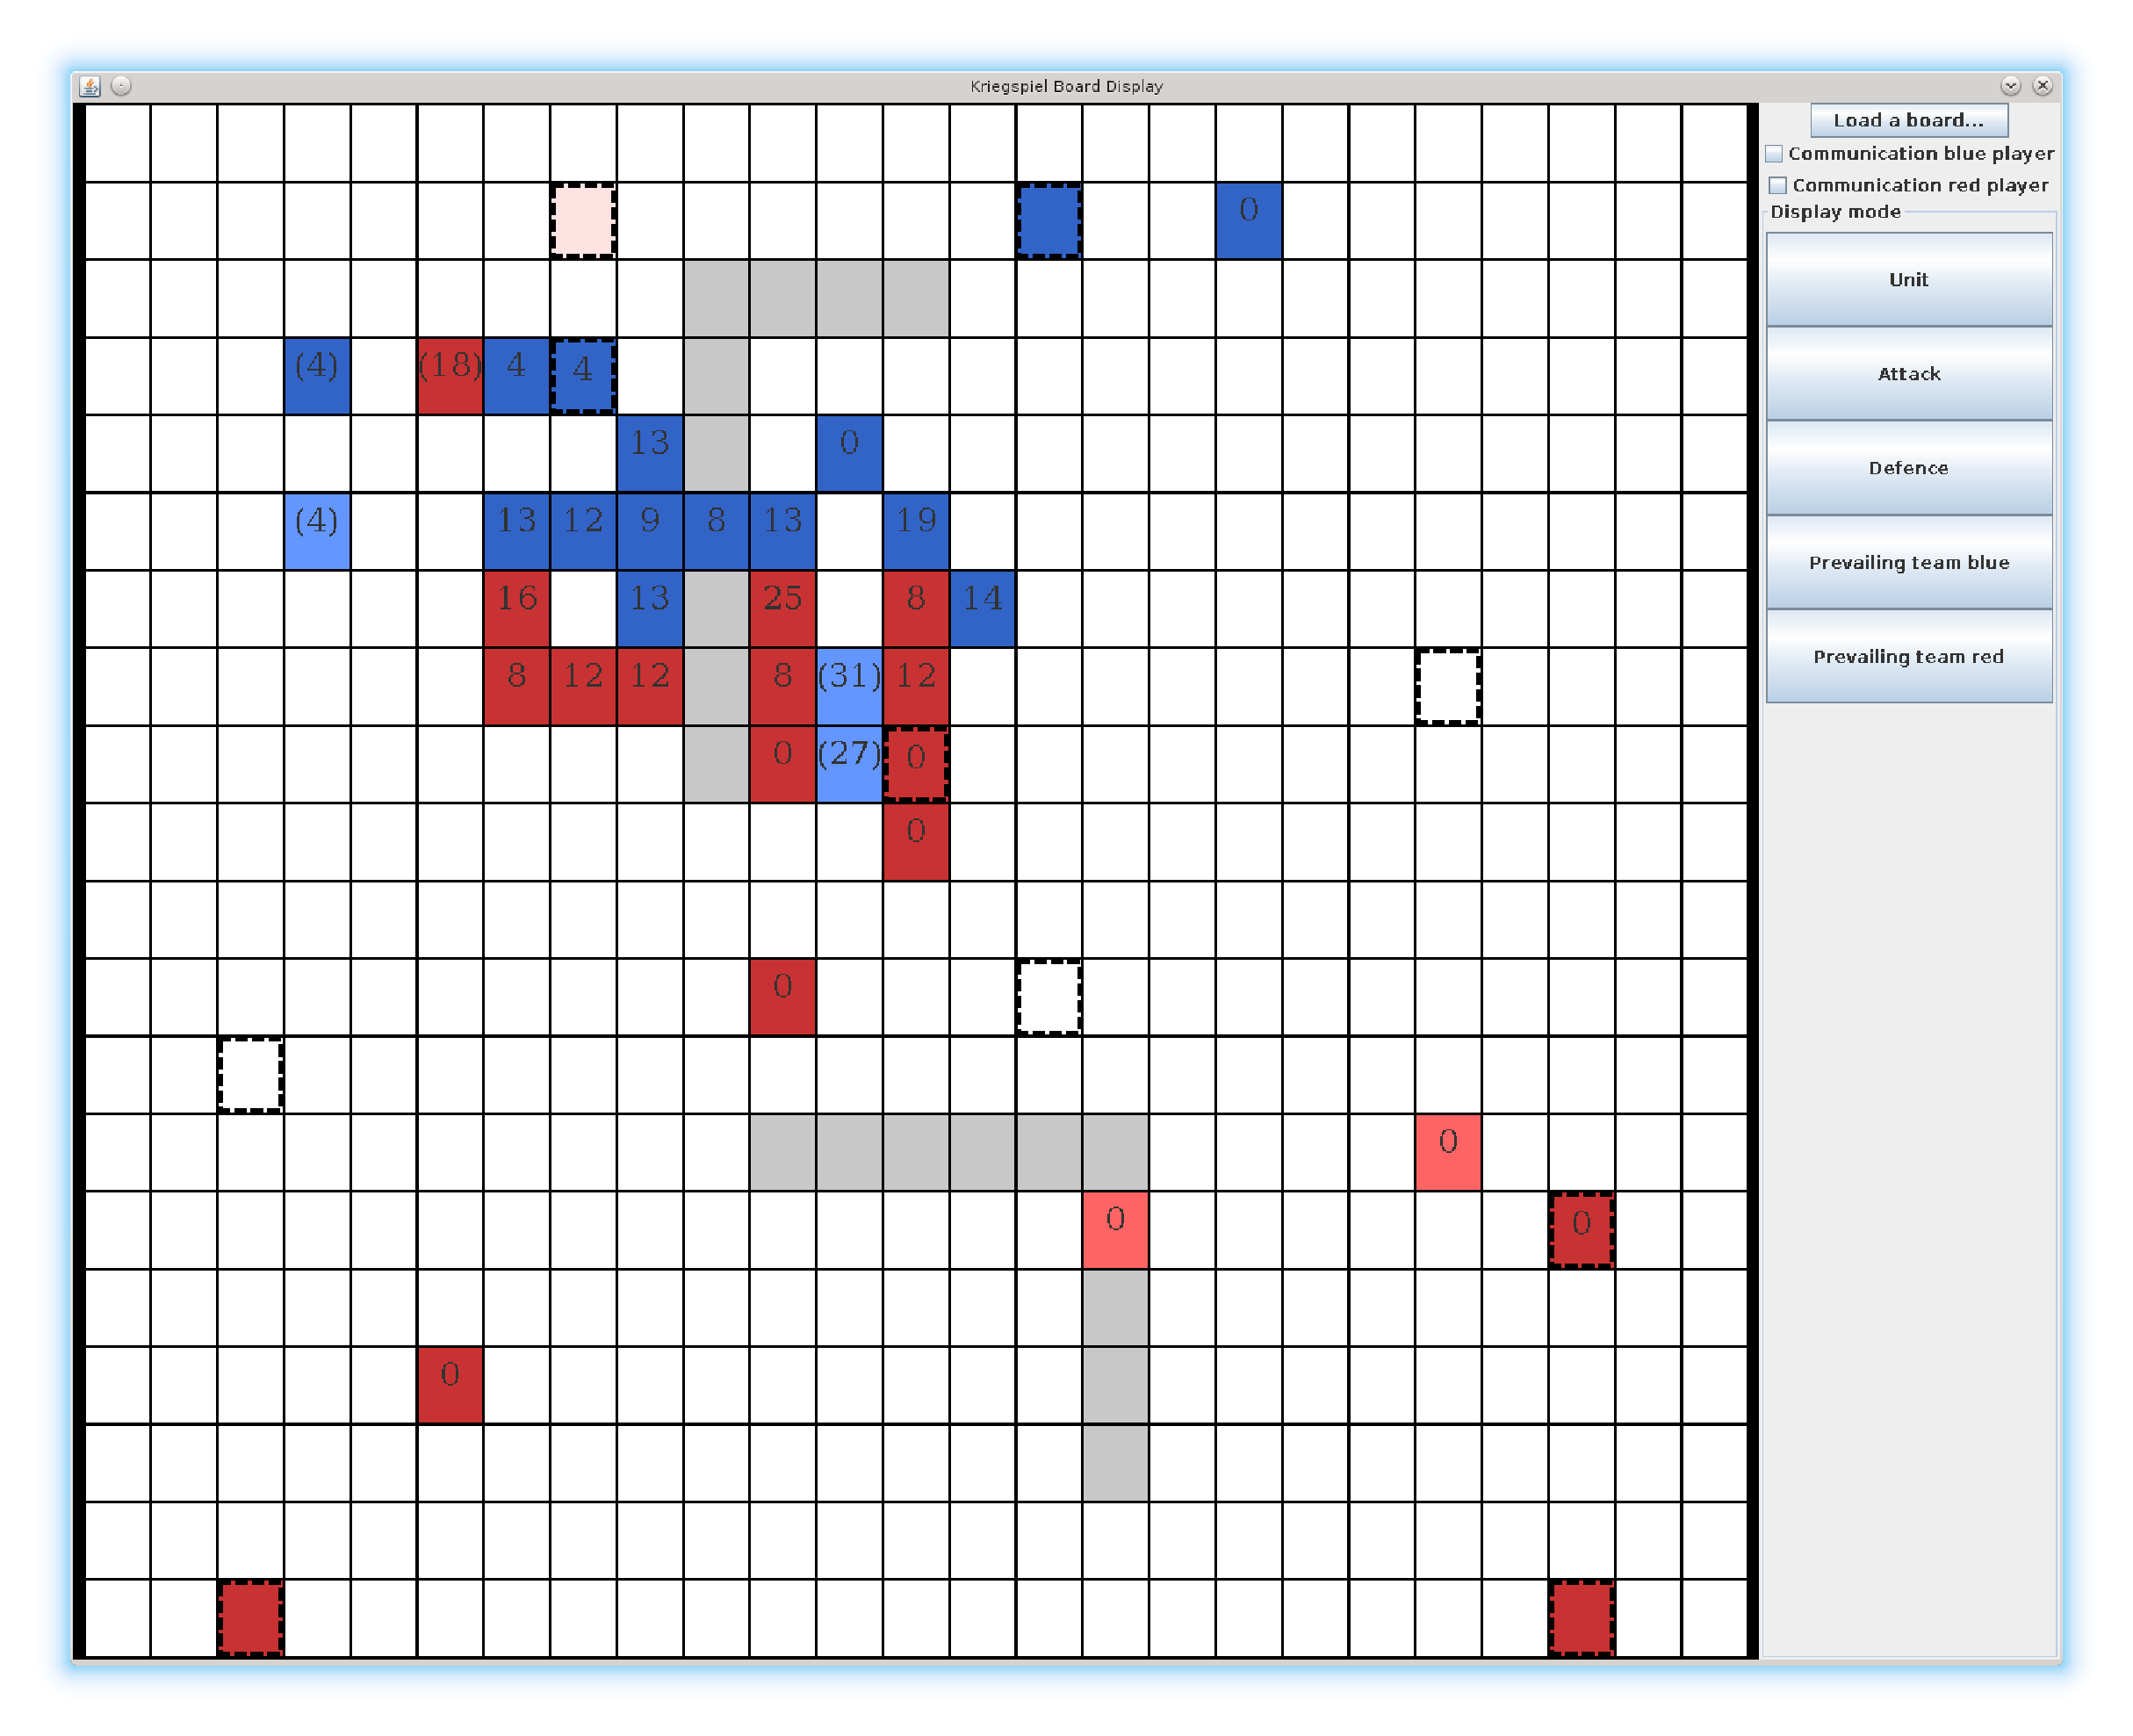
\includegraphics[scale=0.4]{images/screen2.eps}
			Dans le mode attaque, le total d'attaque potentiel est affiché sur chaque unité.
			Dans le mode défense, le total de défense de l'unité est affiché.
		
			\clearpage	

		\subsection{Mode prédominance}
			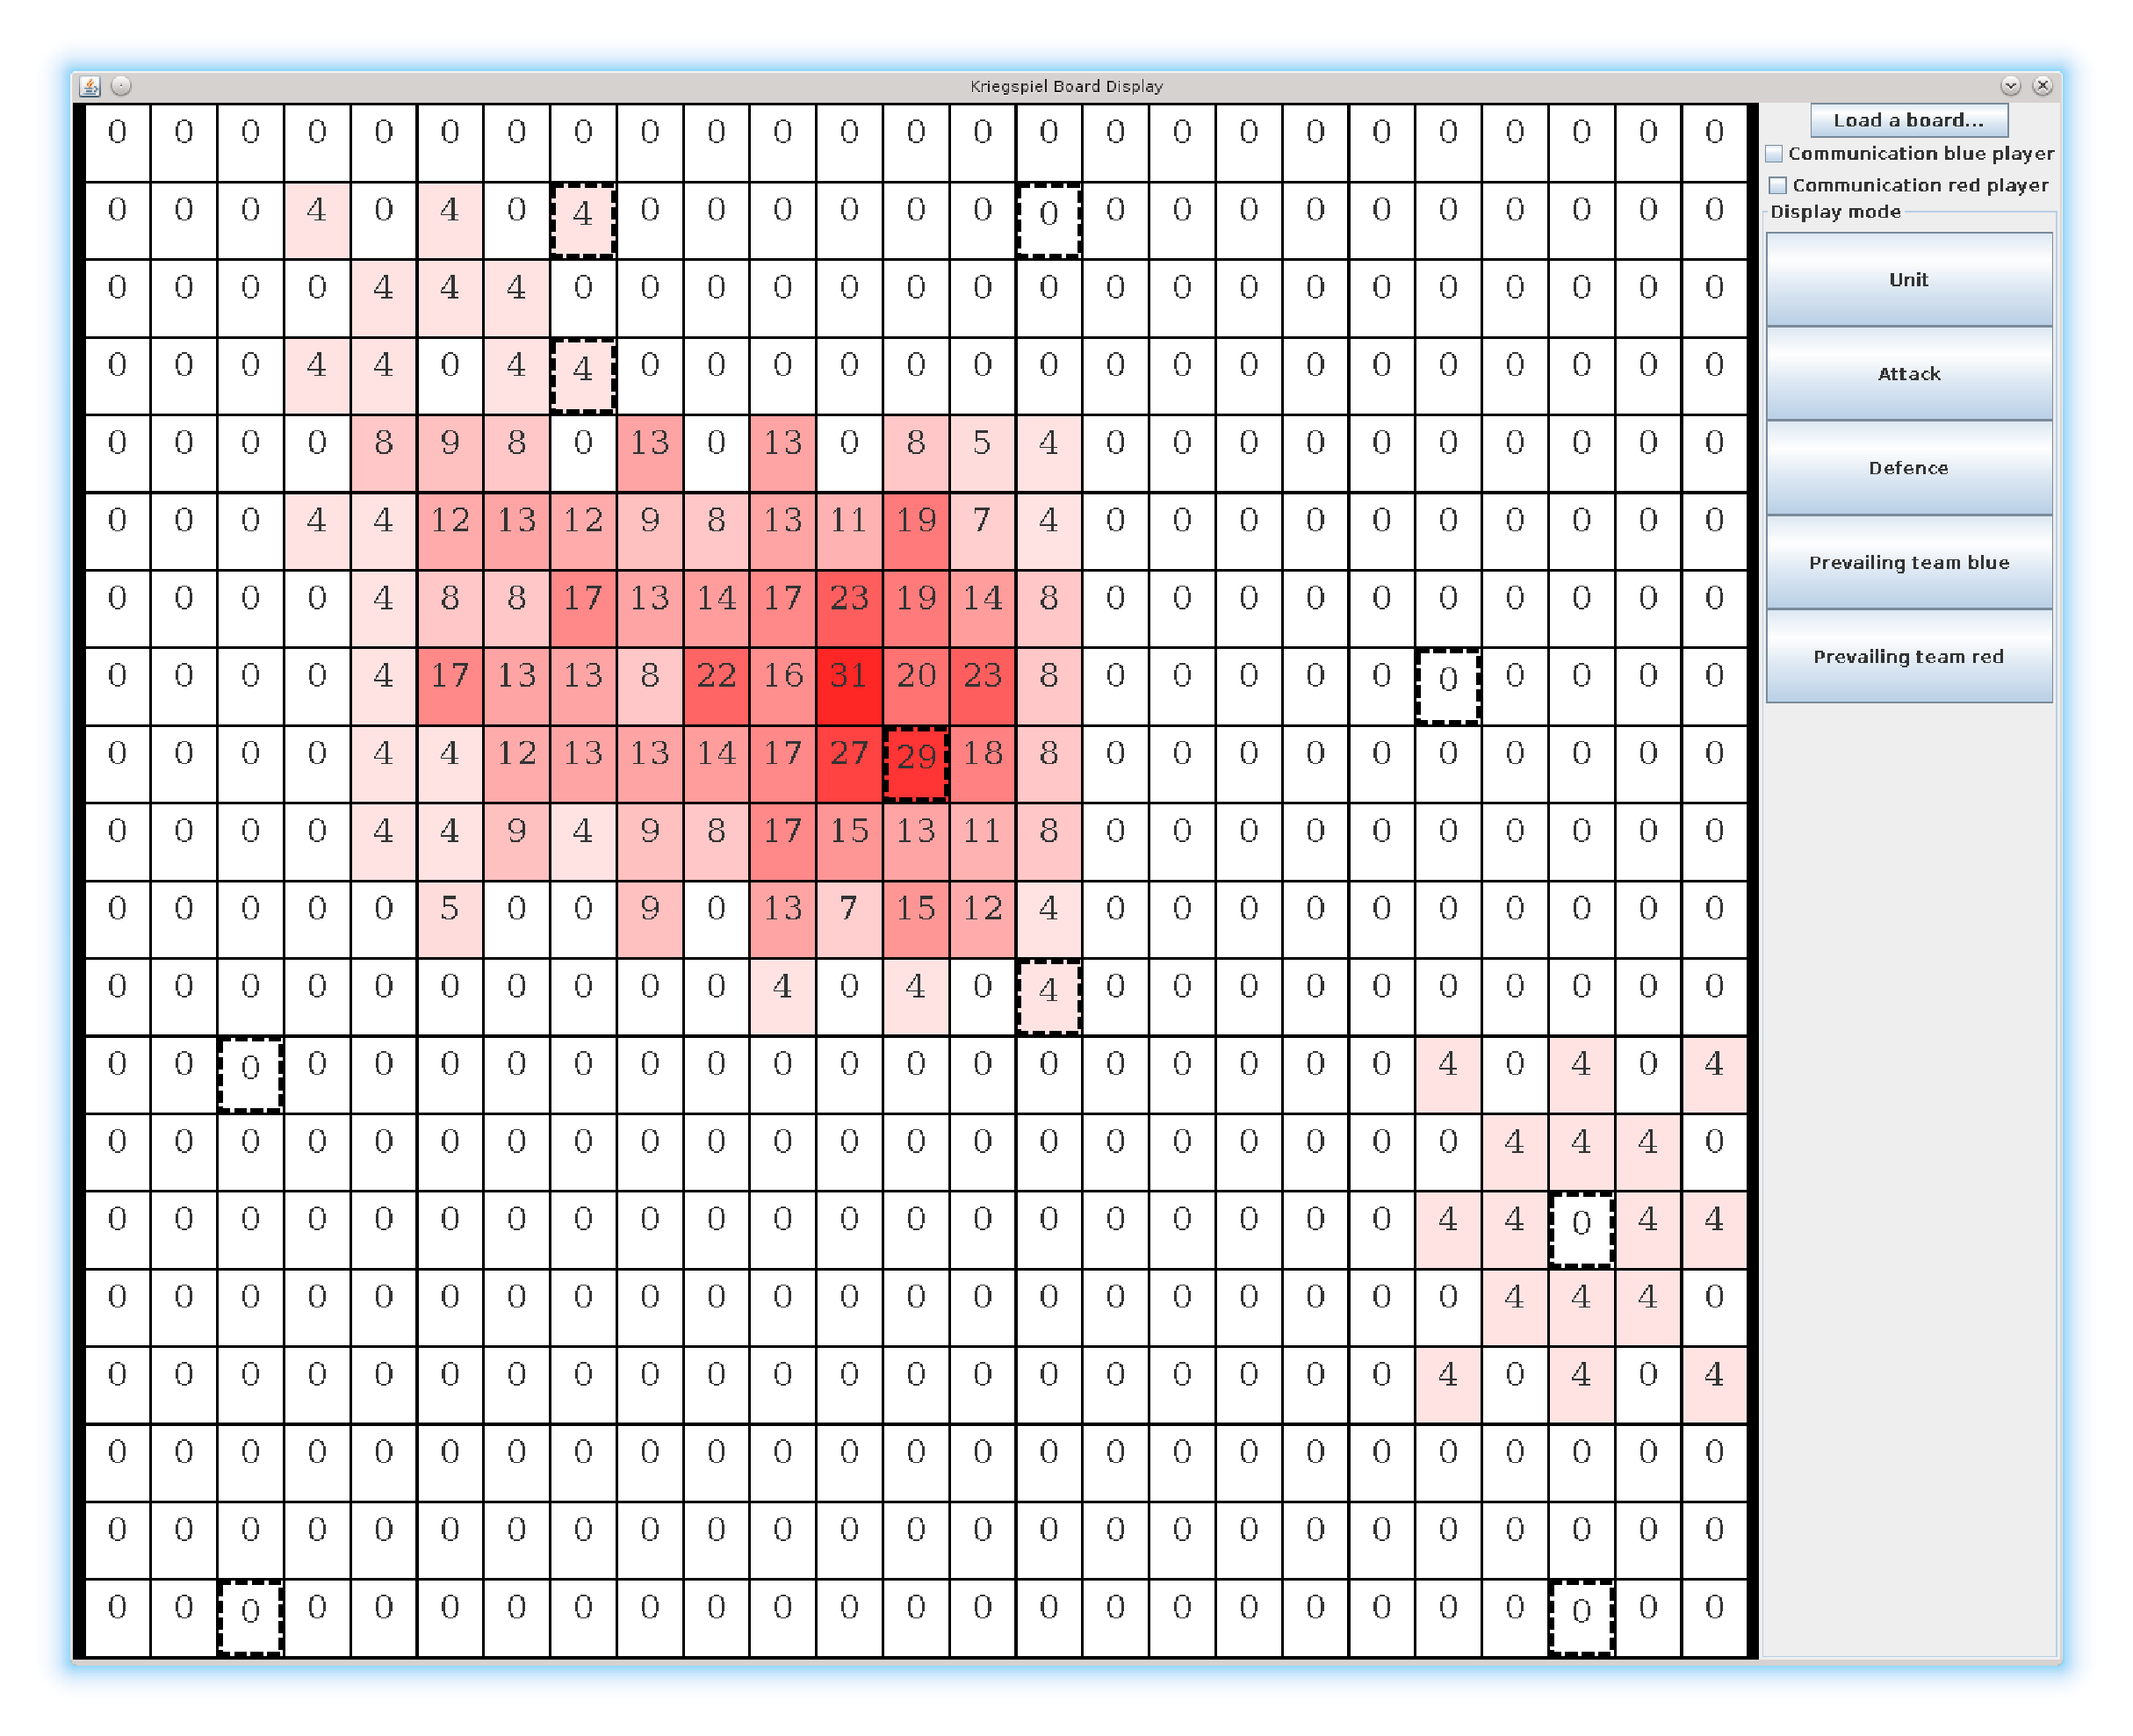
\includegraphics[scale=0.4]{images/screen3.eps}
			Dans le mode prédominance, la matrice de prédominance du joueur choisi est affichée.

			\clearpage

	\section{Autres fonctionnalités}

		\subsection{Lignes de communication}
			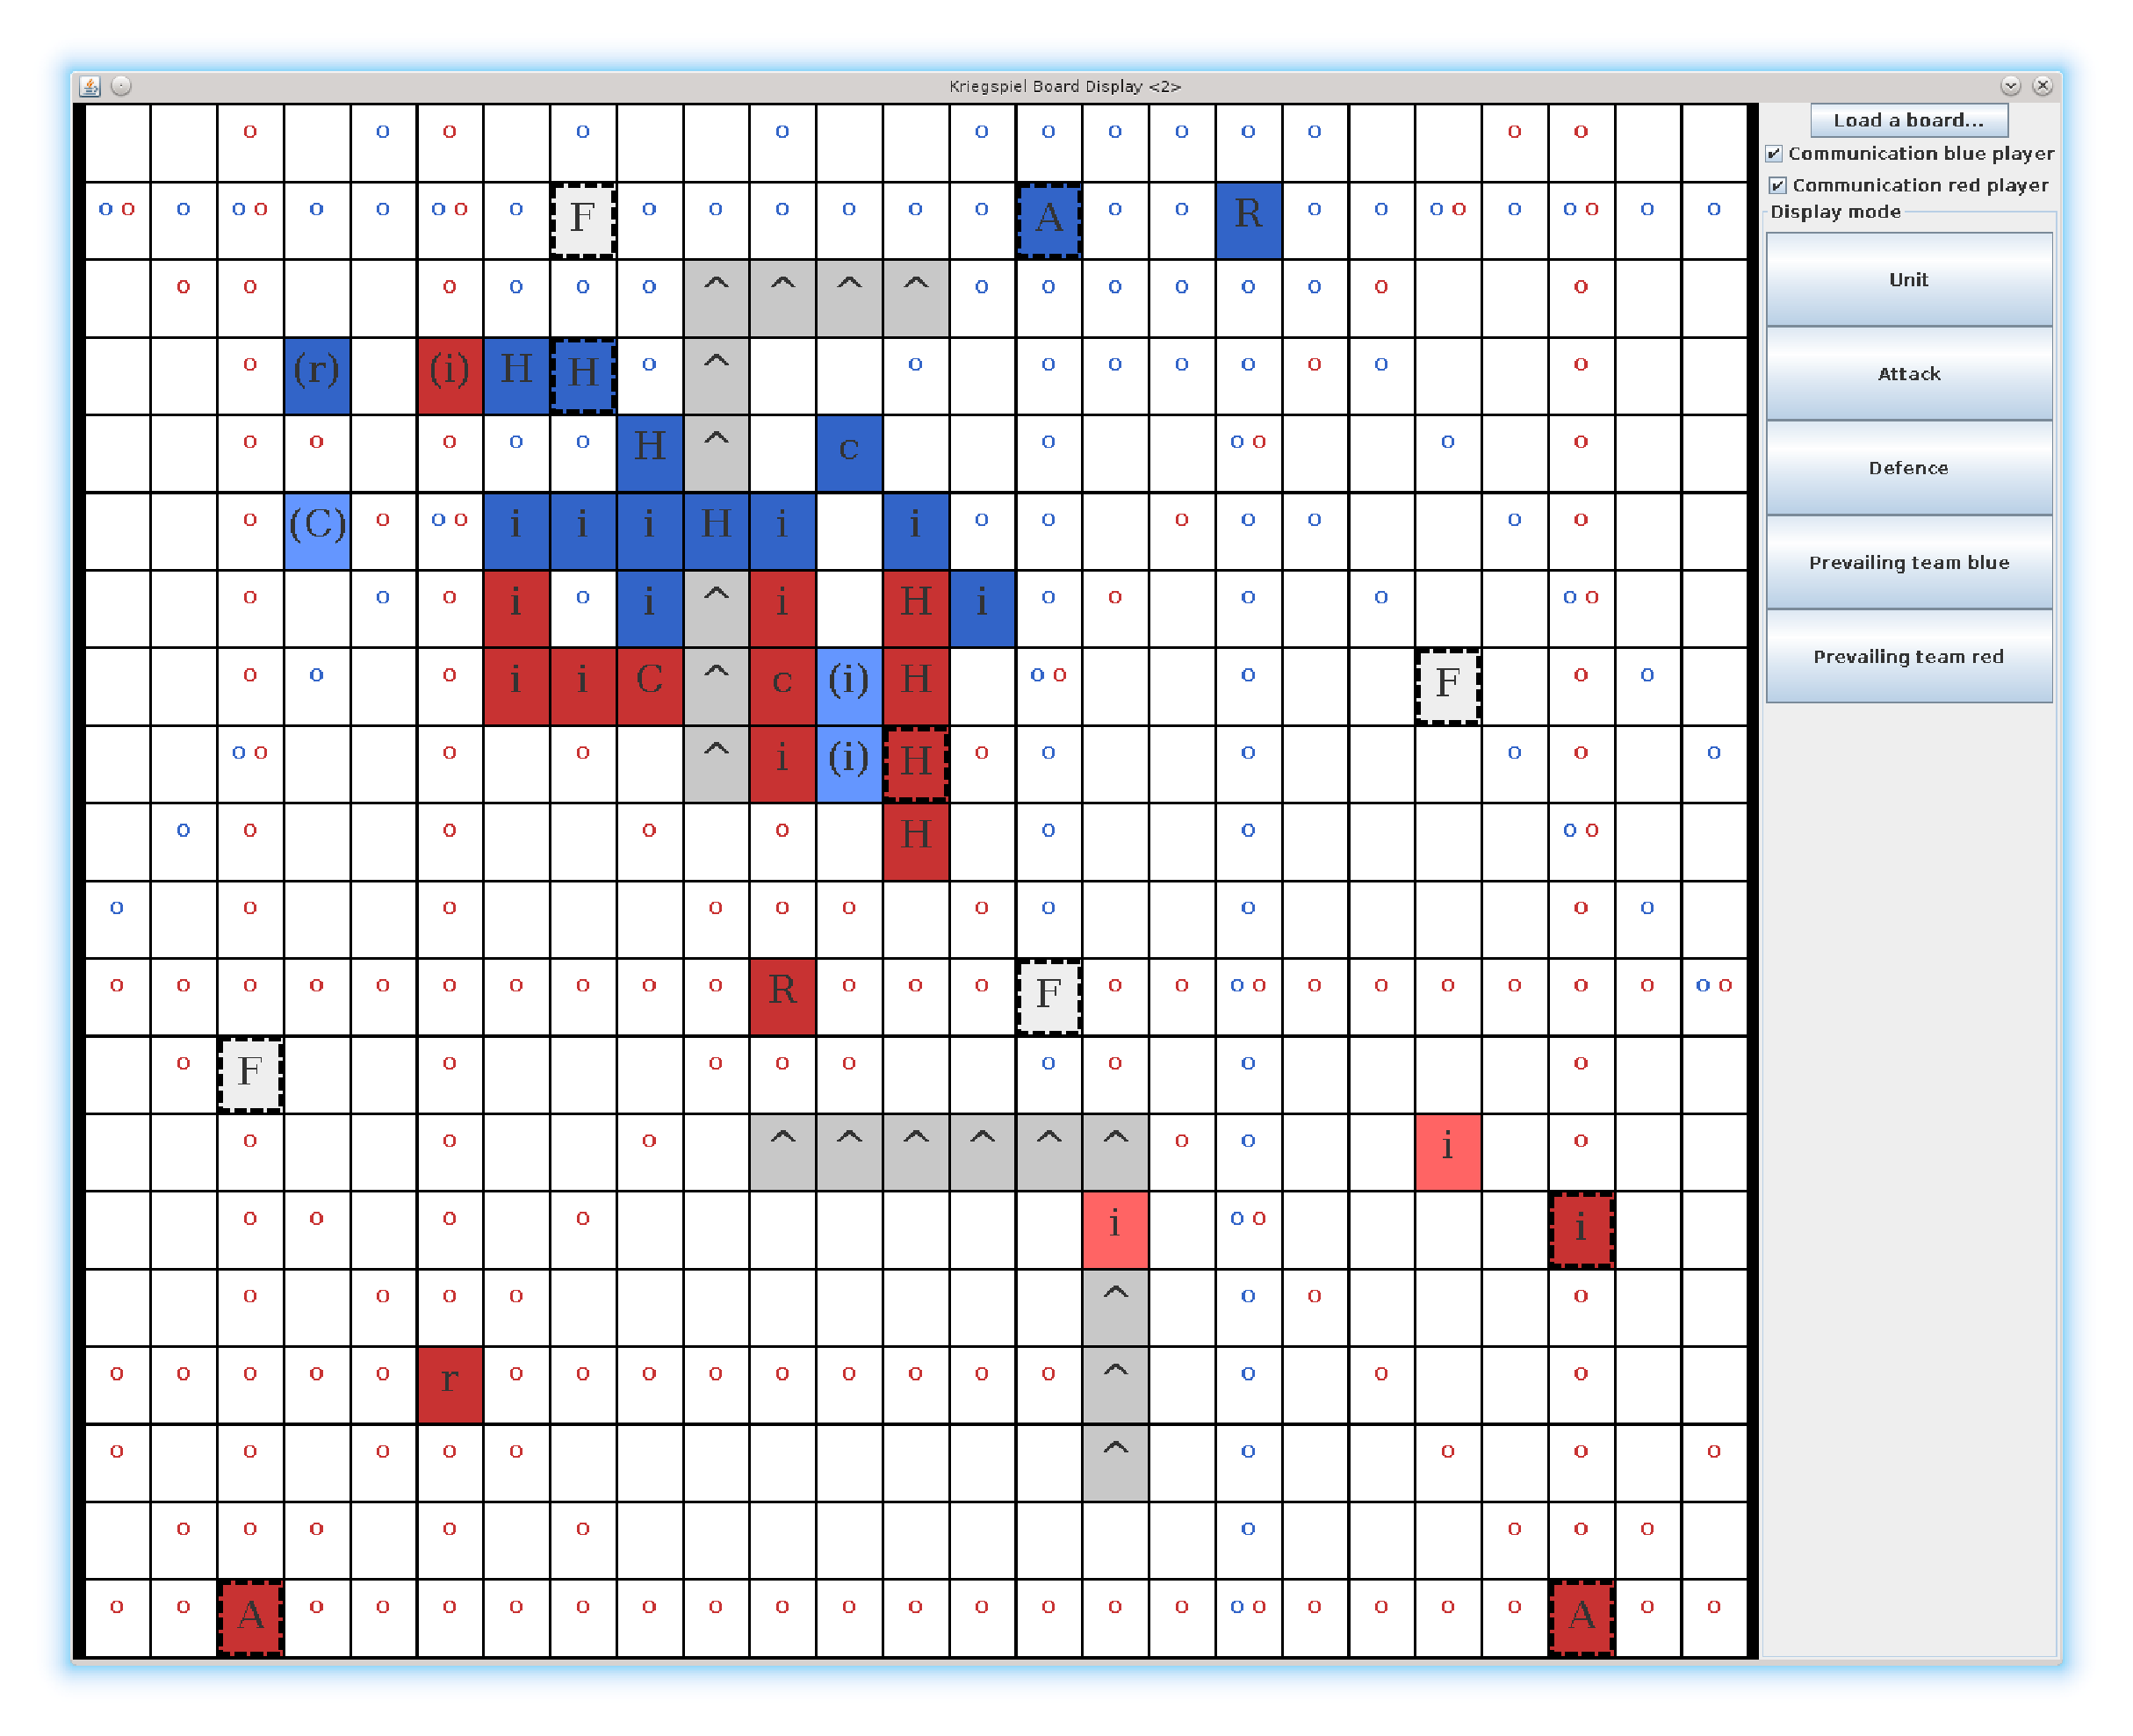
\includegraphics[scale=0.4]{images/screen4.eps}
			Les lignes de communication sont représentées par des cercles de la couleur de l'équipe.
			Les unités déconnectées ont une teinte plus claire que les unités connectées.
			On peut remarquer que les unités adverses bloquent les communications et que les relais alliés les propagent.

			\clearpage